\documentclass{standalone}
\usepackage{tikz}
\usetikzlibrary{patterns}
\usetikzlibrary{positioning}
\usetikzlibrary{patterns, positioning}
\usetikzlibrary{shapes.misc}
\usepackage[outline]{contour}
\contourlength{1.5pt} 
\usepackage[sfdefault]{ClearSans}

\begin{document}
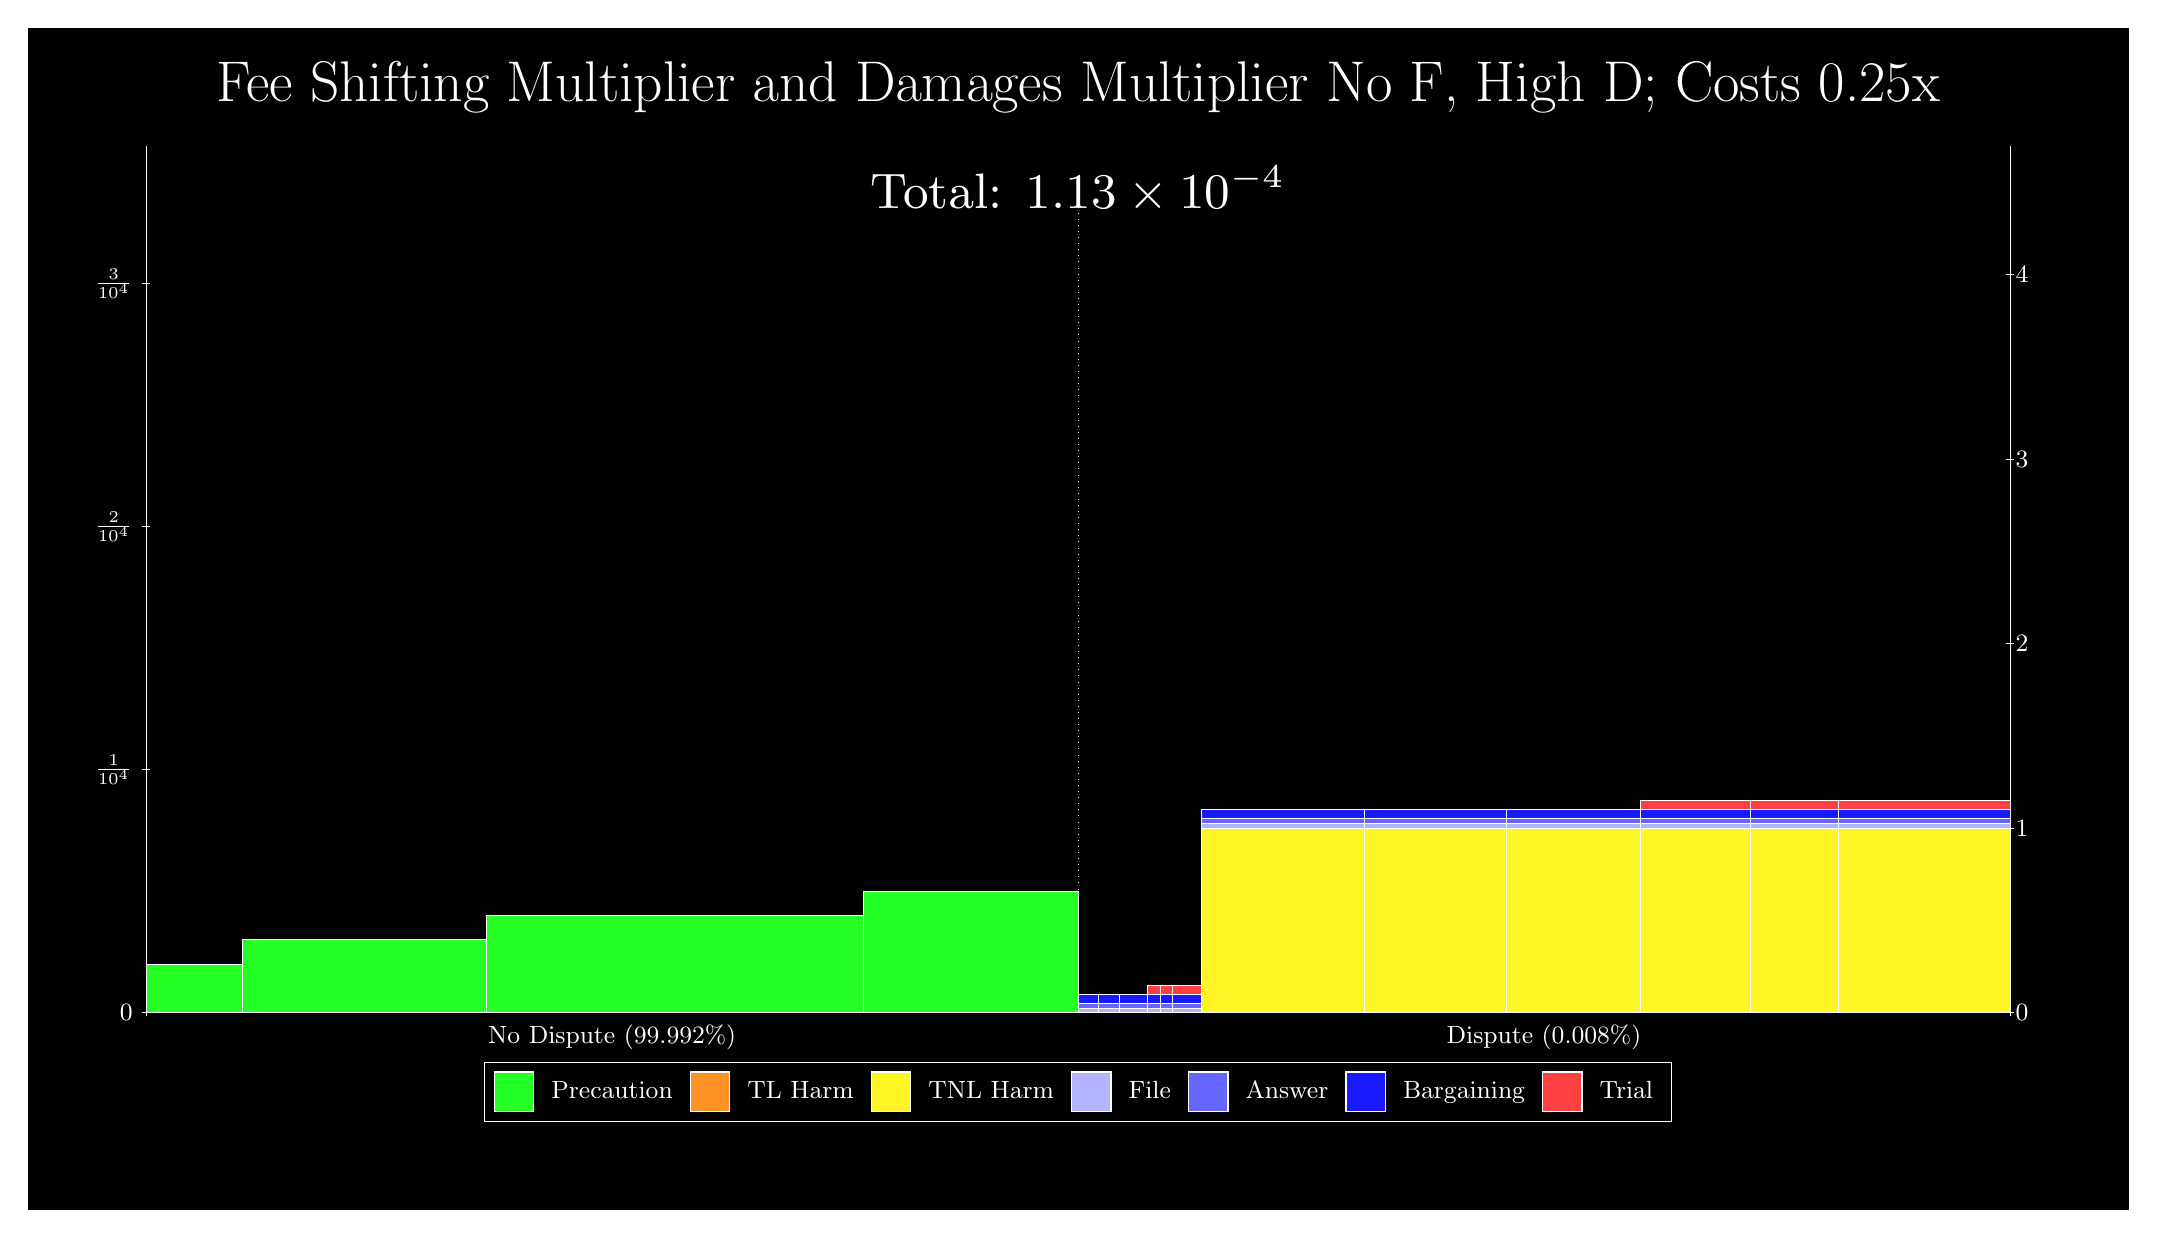
\begin{tikzpicture}
\draw[fill=black] (0,0) rectangle (26.667,15);
\draw[draw=none,text=white] (0,13.5) rectangle (26.667,15) node[midway] {\huge Fee Shifting Multiplier and Damages Multiplier No F, High D; Costs 0.25x};
\draw[fill=green!85,draw=white,very thin] (1.5,2.5) rectangle (2.7168,3.1172);
\draw[fill=green!85,draw=white,very thin] (2.7168,2.5) rectangle (5.8206,3.4257);
\draw[fill=green!85,draw=white,very thin] (5.8206,2.5) rectangle (10.611,3.7343);
\draw[fill=green!85,draw=white,very thin] (10.611,2.5) rectangle (13.333,4.0429);
\draw[fill=green!85,draw=white,very thin] (13.333,2.5) rectangle (13.591,2.5001);
\draw[fill=blue!30,draw=white,very thin] (13.333,2.5001) rectangle (13.591,2.5586);
\draw[fill=blue!60,draw=white,very thin] (13.333,2.5586) rectangle (13.591,2.6172);
\draw[fill=blue!90,draw=white,very thin] (13.333,2.6172) rectangle (13.591,2.7344);
\draw[fill=green!85,draw=white,very thin] (13.591,2.5) rectangle (13.854,2.5001);
\draw[fill=blue!30,draw=white,very thin] (13.591,2.5001) rectangle (13.854,2.5587);
\draw[fill=blue!60,draw=white,very thin] (13.591,2.5587) rectangle (13.854,2.6172);
\draw[fill=blue!90,draw=white,very thin] (13.591,2.6172) rectangle (13.854,2.7344);
\draw[fill=green!85,draw=white,very thin] (13.854,2.5) rectangle (14.216,2.5001);
\draw[fill=blue!30,draw=white,very thin] (13.854,2.5001) rectangle (14.216,2.5587);
\draw[fill=blue!60,draw=white,very thin] (13.854,2.5587) rectangle (14.216,2.6173);
\draw[fill=blue!90,draw=white,very thin] (13.854,2.6173) rectangle (14.216,2.7344);
\draw[fill=green!85,draw=white,very thin] (14.216,2.5) rectangle (14.376,2.5);
\draw[fill=blue!30,draw=white,very thin] (14.216,2.5) rectangle (14.376,2.5586);
\draw[fill=blue!60,draw=white,very thin] (14.216,2.5586) rectangle (14.376,2.6172);
\draw[fill=blue!90,draw=white,very thin] (14.216,2.6172) rectangle (14.376,2.7343);
\draw[fill=red!75,draw=white,very thin] (14.216,2.7343) rectangle (14.376,2.8515);
\draw[fill=green!85,draw=white,very thin] (14.376,2.5) rectangle (14.526,2.5001);
\draw[fill=blue!30,draw=white,very thin] (14.376,2.5001) rectangle (14.526,2.5586);
\draw[fill=blue!60,draw=white,very thin] (14.376,2.5586) rectangle (14.526,2.6172);
\draw[fill=blue!90,draw=white,very thin] (14.376,2.6172) rectangle (14.526,2.7344);
\draw[fill=red!75,draw=white,very thin] (14.376,2.7344) rectangle (14.526,2.8515);
\draw[fill=green!85,draw=white,very thin] (14.526,2.5) rectangle (14.895,2.5001);
\draw[fill=blue!30,draw=white,very thin] (14.526,2.5001) rectangle (14.895,2.5587);
\draw[fill=blue!60,draw=white,very thin] (14.526,2.5587) rectangle (14.895,2.6172);
\draw[fill=blue!90,draw=white,very thin] (14.526,2.6172) rectangle (14.895,2.7344);
\draw[fill=red!75,draw=white,very thin] (14.526,2.7344) rectangle (14.895,2.8515);
\draw[fill=green!85,draw=white,very thin] (14.895,2.5) rectangle (16.968,2.5001);
\draw[fill=yellow!85,draw=white,very thin] (14.895,2.5001) rectangle (16.968,4.843);
\draw[fill=blue!30,draw=white,very thin] (14.895,4.843) rectangle (16.968,4.9016);
\draw[fill=blue!60,draw=white,very thin] (14.895,4.9016) rectangle (16.968,4.9601);
\draw[fill=blue!90,draw=white,very thin] (14.895,4.9601) rectangle (16.968,5.0773);
\draw[fill=green!85,draw=white,very thin] (16.968,2.5) rectangle (18.773,2.5001);
\draw[fill=yellow!85,draw=white,very thin] (16.968,2.5001) rectangle (18.773,4.843);
\draw[fill=blue!30,draw=white,very thin] (16.968,4.843) rectangle (18.773,4.9016);
\draw[fill=blue!60,draw=white,very thin] (16.968,4.9016) rectangle (18.773,4.9602);
\draw[fill=blue!90,draw=white,very thin] (16.968,4.9602) rectangle (18.773,5.0773);
\draw[fill=green!85,draw=white,very thin] (18.773,2.5) rectangle (20.479,2.5001);
\draw[fill=yellow!85,draw=white,very thin] (18.773,2.5001) rectangle (20.479,4.843);
\draw[fill=blue!30,draw=white,very thin] (18.773,4.843) rectangle (20.479,4.9016);
\draw[fill=blue!60,draw=white,very thin] (18.773,4.9016) rectangle (20.479,4.9602);
\draw[fill=blue!90,draw=white,very thin] (18.773,4.9602) rectangle (20.479,5.0773);
\draw[fill=green!85,draw=white,very thin] (20.479,2.5) rectangle (21.865,2.5);
\draw[fill=yellow!85,draw=white,very thin] (20.479,2.5) rectangle (21.865,4.843);
\draw[fill=blue!30,draw=white,very thin] (20.479,4.843) rectangle (21.865,4.9015);
\draw[fill=blue!60,draw=white,very thin] (20.479,4.9015) rectangle (21.865,4.9601);
\draw[fill=blue!90,draw=white,very thin] (20.479,4.9601) rectangle (21.865,5.0773);
\draw[fill=red!75,draw=white,very thin] (20.479,5.0773) rectangle (21.865,5.1944);
\draw[fill=green!85,draw=white,very thin] (21.865,2.5) rectangle (22.984,2.5001);
\draw[fill=yellow!85,draw=white,very thin] (21.865,2.5001) rectangle (22.984,4.843);
\draw[fill=blue!30,draw=white,very thin] (21.865,4.843) rectangle (22.984,4.9016);
\draw[fill=blue!60,draw=white,very thin] (21.865,4.9016) rectangle (22.984,4.9601);
\draw[fill=blue!90,draw=white,very thin] (21.865,4.9601) rectangle (22.984,5.0773);
\draw[fill=red!75,draw=white,very thin] (21.865,5.0773) rectangle (22.984,5.1944);
\draw[fill=green!85,draw=white,very thin] (22.984,2.5) rectangle (22.987,2.5001);
\draw[fill=orange!85,draw=white,very thin] (22.984,2.5001) rectangle (22.987,4.843);
\draw[fill=blue!30,draw=white,very thin] (22.984,4.843) rectangle (22.987,4.9016);
\draw[fill=blue!60,draw=white,very thin] (22.984,4.9016) rectangle (22.987,4.9601);
\draw[fill=blue!90,draw=white,very thin] (22.984,4.9601) rectangle (22.987,5.0773);
\draw[fill=red!75,draw=white,very thin] (22.984,5.0773) rectangle (22.987,5.1944);
\draw[fill=green!85,draw=white,very thin] (22.987,2.5) rectangle (25.167,2.5001);
\draw[fill=yellow!85,draw=white,very thin] (22.987,2.5001) rectangle (25.167,4.843);
\draw[fill=blue!30,draw=white,very thin] (22.987,4.843) rectangle (25.167,4.9016);
\draw[fill=blue!60,draw=white,very thin] (22.987,4.9016) rectangle (25.167,4.9602);
\draw[fill=blue!90,draw=white,very thin] (22.987,4.9602) rectangle (25.167,5.0773);
\draw[fill=red!75,draw=white,very thin] (22.987,5.0773) rectangle (25.167,5.1945);
\node[font=\small,text=white,anchor=north,scale=2] at (13.333, 13.5) {Total: $1.13\times 10^{-4}$};
\draw[white,very thin] (1.5,2.5) -- (1.5,13.5);
\draw[white,very thin] (1.45,2.5) -- (1.55,2.5);
\node[font=\small,text=white, anchor=east] at (1.45, 2.5) {0};
\draw[white,very thin] (1.45,5.5858) -- (1.55,5.5858);
\node[font=\small,text=white, anchor=east] at (1.45, 5.5858) {$\frac{1}{10^{4}}$};
\draw[white,very thin] (1.45,8.6715) -- (1.55,8.6715);
\node[font=\small,text=white, anchor=east] at (1.45, 8.6715) {$\frac{2}{10^{4}}$};
\draw[white,very thin] (1.45,11.757) -- (1.55,11.757);
\node[font=\small,text=white, anchor=east] at (1.45, 11.757) {$\frac{3}{10^{4}}$};

\draw[white,dotted,very thin] (13.333,2.83) -- (13.333,13.17);
\draw[white,very thin] (25.167,2.5) -- (25.167,13.5);
\draw[white,very thin] (25.117,2.5) -- (25.217,2.5);
\node[font=\small,text=white, anchor=west] at (25.117, 2.5) {0};
\draw[white,very thin] (25.117,4.8429) -- (25.217,4.8429);
\node[font=\small,text=white, anchor=west] at (25.117, 4.8429) {1};
\draw[white,very thin] (25.117,7.1859) -- (25.217,7.1859);
\node[font=\small,text=white, anchor=west] at (25.117, 7.1859) {2};
\draw[white,very thin] (25.117,9.5288) -- (25.217,9.5288);
\node[font=\small,text=white, anchor=west] at (25.117, 9.5288) {3};
\draw[white,very thin] (25.117,11.872) -- (25.217,11.872);
\node[font=\small,text=white, anchor=west] at (25.117, 11.872) {4};

\draw[white,very thin] (1.5,2.5) -- (25.167,2.5);
\draw[white,very thin] (1.5,2.45) -- (1.5,2.55);
\node[font=\small,text=white, anchor=north] at (1.5, 2.45) {};
\draw[white,very thin] (25.167,2.45) -- (25.167,2.55);
\node[font=\small,text=white, anchor=north] at (25.167, 2.45) {};

\node[font=\small,text=white,anchor=south] at (7.4167, 1.9) {No\ Dispute\ (99.992\%)};
\node[font=\small,text=white,anchor=south] at (19.25, 1.9) {Dispute\ (0.008\%)};
\draw (13.3333,2.5) node (B) {};
\begin{scope}[align=center]
\matrix[scale=0.5,draw=white,below=0.5cm of B,nodes={draw},column sep=0.1cm]{
\node[rectangle,draw,minimum width=0.5cm,minimum height=0.5cm,fill=green!85]{}; & \node[draw=none,font=\small,text=white]{Precaution}; &
\node[rectangle,draw,minimum width=0.5cm,minimum height=0.5cm,fill=orange!85]{}; & \node[draw=none,font=\small,text=white]{TL Harm}; &
\node[rectangle,draw,minimum width=0.5cm,minimum height=0.5cm,fill=yellow!85]{}; & \node[draw=none,font=\small,text=white]{TNL Harm}; &
\node[rectangle,draw,minimum width=0.5cm,minimum height=0.5cm,fill=blue!30]{}; & \node[draw=none,font=\small,text=white]{File}; &
\node[rectangle,draw,minimum width=0.5cm,minimum height=0.5cm,fill=blue!60]{}; & \node[draw=none,font=\small,text=white]{Answer}; &
\node[rectangle,draw,minimum width=0.5cm,minimum height=0.5cm,fill=blue!90]{}; & \node[draw=none,font=\small,text=white]{Bargaining}; &
\node[rectangle,draw,minimum width=0.5cm,minimum height=0.5cm,fill=red!75]{}; & \node[draw=none,font=\small,text=white]{Trial}; \\\\
};\end{scope}

\end{tikzpicture}
\end{document}